\section{Data collection} \label{sec:data_collection}
\subsection{Implementations}
The purpose of collecting our own dataset is to investigate the impacts of diverse settings on the synthesized target views.
This dataset has to cover a wide variety of usage scenarios with: (i) different camera placement strategies, (ii) random target view trajectories mimicking real HMD users, (iii) scenes with diverse characteristics (e.g., lighting conditions, color tone, and dynamics), we capture the source views by extending AirSim~\cite{airsim}, which is an open source project that provides Application Programming Interface (API) for programmers.
For example, we develop tools using camera control API to capture source views.
Moreover, we adopt the random waypoint as the mobility model to generate random target view trajectories.
In addition to random trajectories, we also implement tools to collect real HMD user trajectories using Unreal Engine.
In a pilot test, we recruit three HMD users, play a random scene to them, and analyze their target view trajectories.
We found that the dynamic ranges of roll/pitch/yaw are 80/80/100 degrees, and the angular velocity is between 8 and 80 degree/s.
We also found the HMD users moves at a speed between 0.1 and 1 m/s.
We use these statistics to generate random target view trajectories. 

\begin{figure*}[tbh]
    \centering
    \subfigure[]{
        \label{fig:screenshot_LightRoomDemo}
        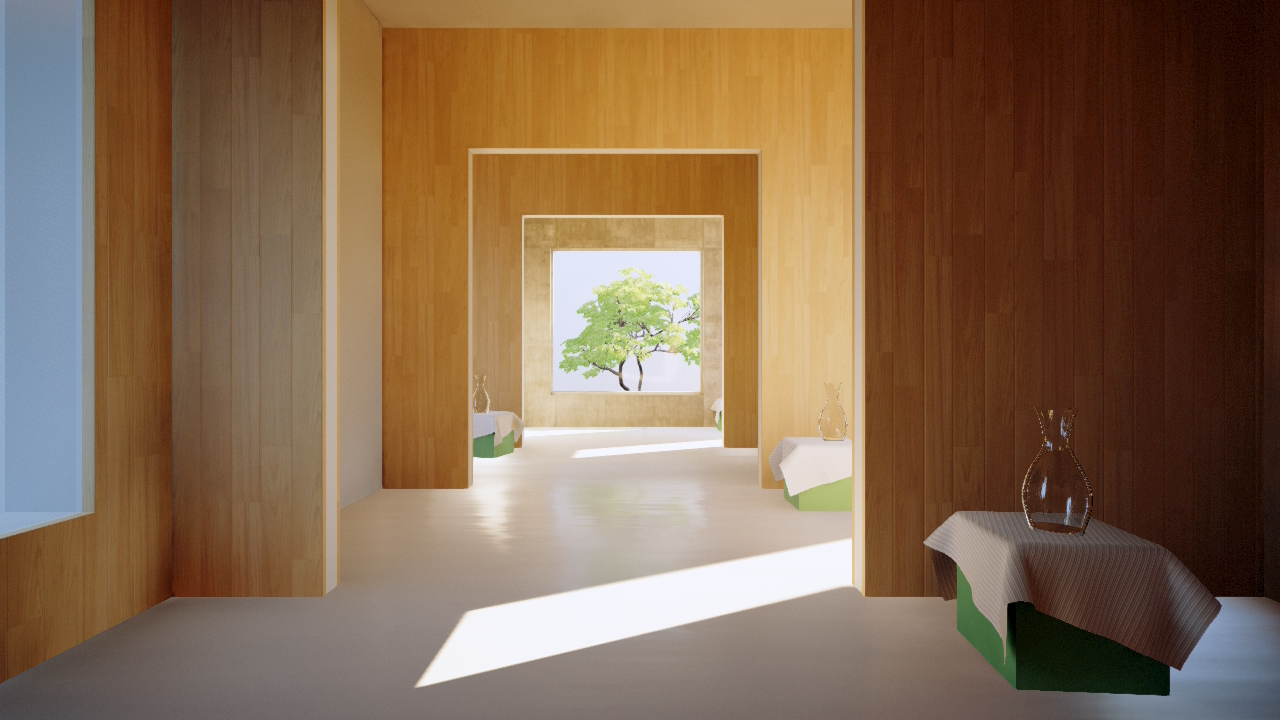
\includegraphics[width=.18\textwidth]{figs/screenshot/LightRoomDemo.png}
    }
    \subfigure[]{
        \label{fig:screenshot_ArchDemo}
        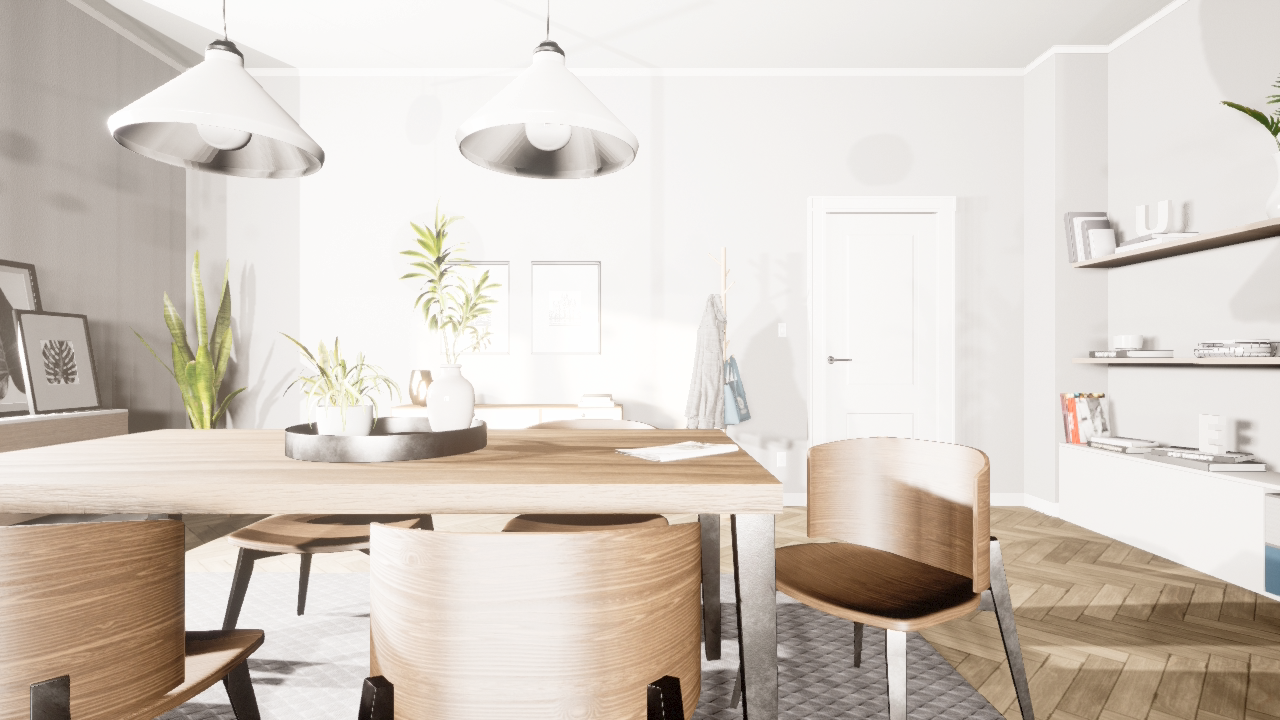
\includegraphics[width=.18\textwidth]{figs/screenshot/ArchDemo.png}
    }
    \subfigure[]{
        \label{fig:screenshot_XoioDemo}
        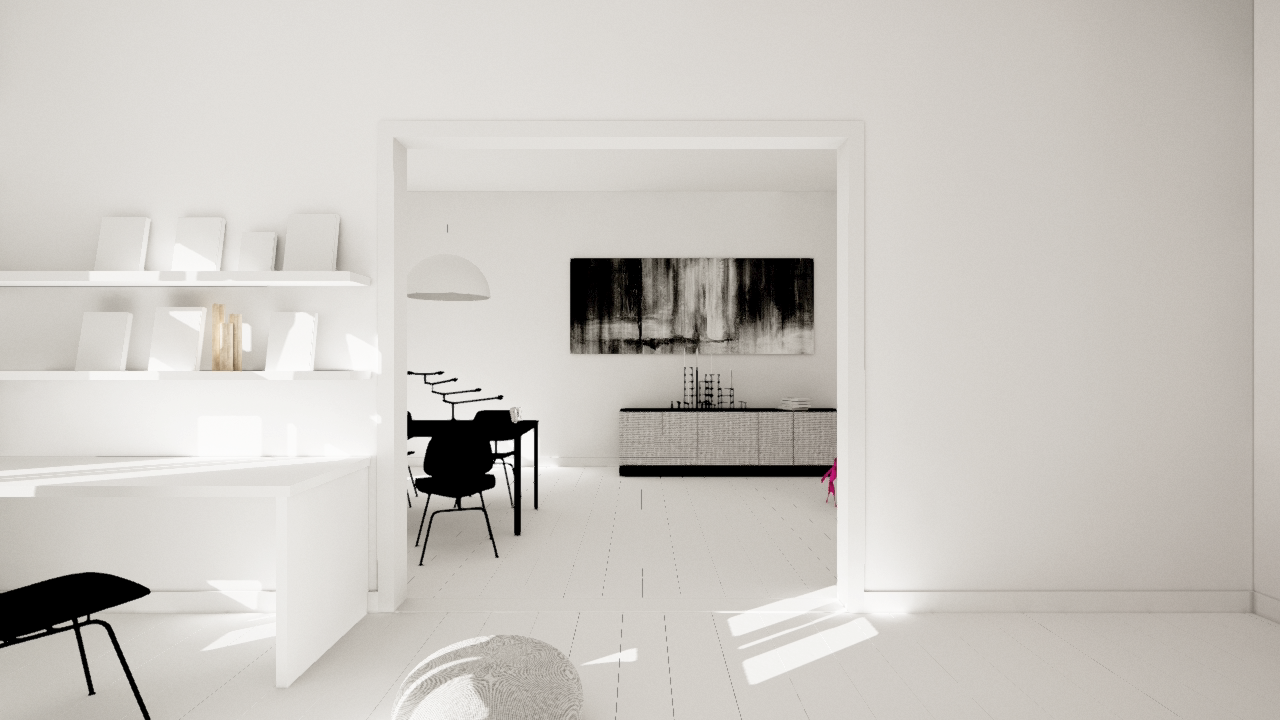
\includegraphics[width=.18\textwidth]{figs/screenshot/XoioDemo.png}
    }
    \subfigure[]{
        \label{fig:screenshot_OfficeDemo}
        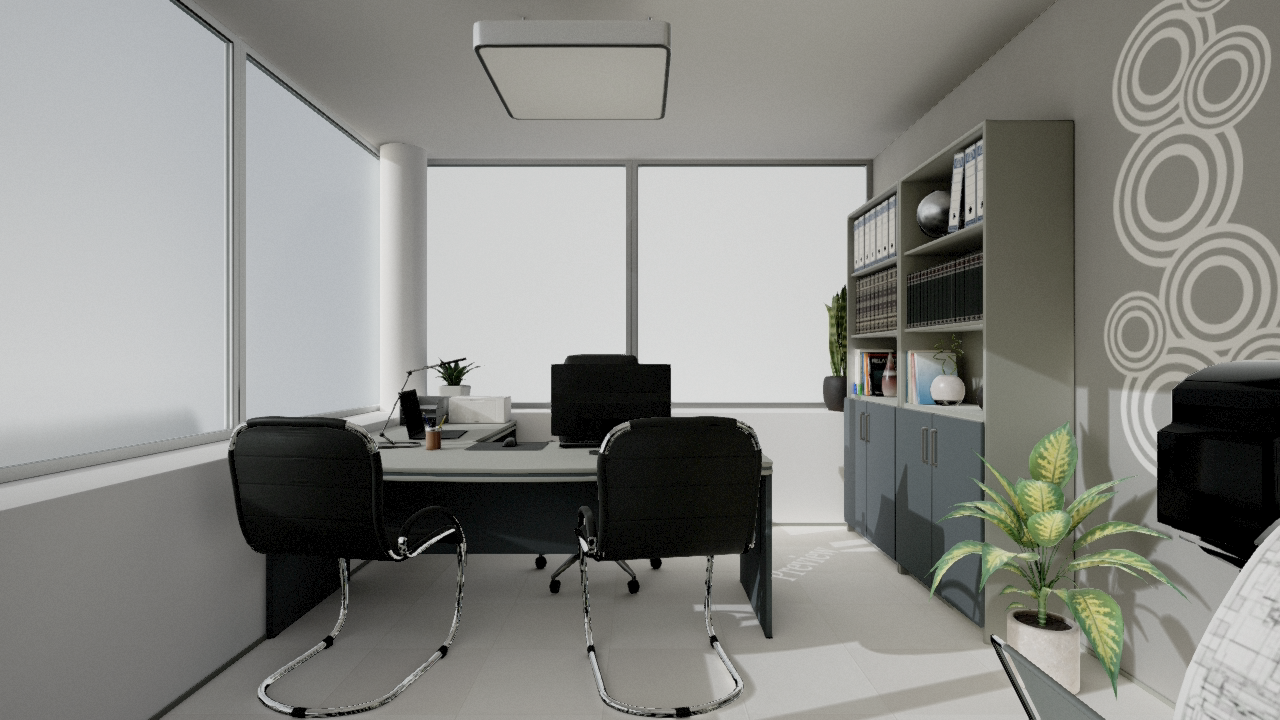
\includegraphics[width=.18\textwidth]{figs/screenshot/OfficeDemo.png}
    }
    \subfigure[]{
        \label{fig:screenshot_RealisticDemo}
        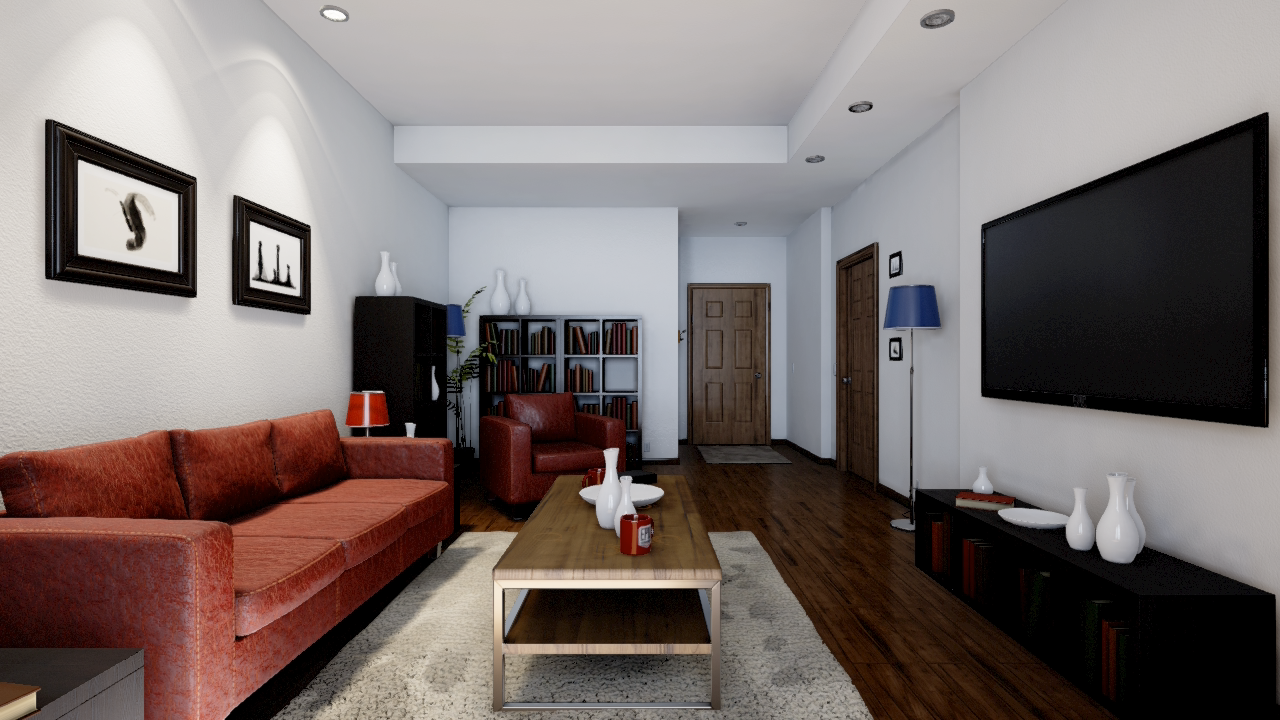
\includegraphics[width=.18\textwidth]{figs/screenshot/RealisticDemo.png}
    }
    \caption{The considered scenes sorted in increasing complexity levels: (a) {\em Light}, 
    (b) {\em Arch}, (c) {\em Xoio}, (d) {\em Office}, and (e) {\em Real}.}
    \label{fig:screenshot}
\end{figure*}

\subsection{The Dataset} \label{ssec:dataset}
We select five scenes from Unreal Engine marketplace~\cite{UE_marketplace}, and modify one of them into a dynamic scene. 
Fig.~\ref{fig:screenshot} gives sample video frame of these scenes (except the dynamic one). 
Table~\ref{tab:sceneCompare} summarizes the scenes with key characteristics. 
The synthesized target views from these scenes exhibit different complexities in terms of Temporal Information (TI) and Spatial Information (SI). The dynamic scene, {\em RealD}, is generated by adding a howling wolf and a rolling ball to {\em Real}. For each scene, we manually choose direction that have the richest set of visual features. We then place 36 cameras with one of the four placements: 6X6, 9X4, 12X3, and 18X2. Following MPEG's recommendations, all cameras and trajectories are confined in a $0.35 \times 1 \times 1$ $m^{3}$ bounding box. We set the resolution and Field-of-View (FoV) of each camera to be $1280 \times 720$ and 90{\degree}, respectively. We generate 10 target view trajectories: $t_1$ to $t_{10}$ using the random waypoint model. We also selected a real HMD user's trajectory from our pilot test that covers the largest surface of the scene. We refer to it as $u_1$. Each trajectory contains 90 samples of positions and orientations at 30 Hz. 

\begin{table}[hbt]
    \caption{Scenes in Our Dataset}
    \centering
    \resizebox{.46\textwidth}{!}{%
        \begin{tabular}{|c|c|c|c|c|c|c|c|} 
        \hline
        {\bf Scene} & {\bf \# Obj.} & {\bf \# Mesh.} & {\bf Space} & {\bf Lighting} & {\bf Color Tone} & {\bf TI} & {\bf SI}\\
        \hline
        {\bf {\em Light}} & 52 & 51.3 K & Narrow & Bright & Warm & 19.1 & 35.0 \\
        \hline
        {\bf {\em Arch}} & 282 & 5.5 M & Wide & Bright & Warm & 27.1 & 57.4 \\
        \hline
        {\bf {\em Xoio}} & 125 & 2.8 M & Wide & Bright & Cold & 26.2 & 57.8 \\
        \hline
        {\bf {\em Office}} & 96 & 100.4 K & Narrow & Dark & Cold & 29.6 & 62.2 \\
        \hline
        {\bf {\em Real}} & 352 & 221.1 K & Narrow & Medium & Warm & 34.7 & 66.7 \\
        \hline
        % {\bf {\em RealD}} & 354 & 222.1 K & Narrow & Bright & Warm & 32.0 & 58.5 \\
        % \hline
        \end{tabular}
    }
    \label{tab:sceneCompare}
\end{table}

One last complication is the different coordinate systems used by: (i) Unreal Engine (North-Eastern-up, left-handed), (ii) AirSim (North-Eastern-down, right-handed), and (iii) TMIV (North-Western-up, right-handed).
We have implemented scripts to convert the coordinate systems.
For each combination of the scene and camera placement (trajectories), we capture RGBD videos from individual cameras, which are {\em source views}.
We also captured the RGBD video clips following individual target view trajectories, which are {\em target views}, or ground truth.
Both source and target views are stored as raw videos.
In summary, our dataset contains: (i) source view placements (trajectories), (ii) target view (trajectories), (iii) source views, and (iv) target views.
We plan to make our tools and sample dataset public.
